% ============================================================
% Question Bank: ch04-07 Laws of Exponents
% Topic Title: Laws of Exponents
% CCSS: Supplementary (FL, VA)
% Questions: 30 (18 MC + 7 SA + 5 Graphical)
% ============================================================

% --- Multiple Choice Questions (18) ---

\begin{practiceQuestion}{4-7-q01}{mc}
\begin{questionText}
Simplify $3^4 \cdot 3^2$.
\end{questionText}
\choiceA{$3^8$}
\choiceB{$3^6$}
\choiceC{$9^6$}
\choiceD{$3^2$}
\correctAnswer{B}
\explanation{Same base, add exponents: $3^{4+2} = 3^6$.}
\end{practiceQuestion}

\begin{practiceQuestion}{4-7-q02}{mc}
\begin{questionText}
Simplify $\dfrac{5^7}{5^3}$.
\end{questionText}
\choiceA{$5^{10}$}
\choiceB{$5^4$}
\choiceC{$1^4$}
\choiceD{$5^{21}$}
\correctAnswer{B}
\explanation{Same base, subtract exponents: $5^{7-3} = 5^4$.}
\end{practiceQuestion}

\begin{practiceQuestion}{4-7-q03}{mc}
\begin{questionText}
Simplify $(2^3)^4$.
\end{questionText}
\choiceA{$2^7$}
\choiceB{$2^{12}$}
\choiceC{$2^{34}$}
\choiceD{$8^4$}
\correctAnswer{B}
\explanation{Power of a power: multiply exponents. $2^{3 \times 4} = 2^{12}$.}
\end{practiceQuestion}

\begin{practiceQuestion}{4-7-q04}{mc}
\begin{questionText}
What is the value of $9^0$?
\end{questionText}
\choiceA{$0$}
\choiceB{$9$}
\choiceC{$1$}
\choiceD{$-1$}
\correctAnswer{C}
\explanation{Any nonzero number raised to the power of $0$ equals $1$. So $9^0 = 1$.}
\end{practiceQuestion}

\begin{practiceQuestion}{4-7-q05}{mc}
\begin{questionText}
Which expression equals $7^5 \cdot 7^3$?
\end{questionText}
\choiceA{$7^{15}$}
\choiceB{$7^8$}
\choiceC{$49^8$}
\choiceD{$7^2$}
\correctAnswer{B}
\explanation{Product rule: $7^{5+3} = 7^8$.}
\end{practiceQuestion}

\begin{practiceQuestion}{4-7-q06}{mc}
\begin{questionText}
Simplify $\dfrac{10^8}{10^5}$.
\end{questionText}
\choiceA{$10^3 = 1{,}000$}
\choiceB{$10^{13}$}
\choiceC{$10^{40}$}
\choiceD{$1^3$}
\correctAnswer{A}
\explanation{Quotient rule: $10^{8-5} = 10^3 = 1{,}000$.}
\end{practiceQuestion}

\begin{practiceQuestion}{4-7-q07}{mc}
\begin{questionText}
Simplify $(4^2)^3$.
\end{questionText}
\choiceA{$4^5$}
\choiceB{$4^6$}
\choiceC{$4^8$}
\choiceD{$4^{23}$}
\correctAnswer{B}
\explanation{Power of a power: $4^{2 \times 3} = 4^6$.}
\end{practiceQuestion}

\begin{practiceQuestion}{4-7-q08}{mc}
\begin{questionText}
A student writes $2^3 \cdot 3^4 = 6^7$. Is this correct?
\end{questionText}
\choiceA{Yes, you add the exponents}
\choiceB{No, the bases must be the same to use the product rule}
\choiceC{Yes, you multiply the bases and add the exponents}
\choiceD{No, the answer should be $6^{12}$}
\correctAnswer{B}
\explanation{The product rule only works when the bases are the same. $2^3$ and $3^4$ have different bases, so they cannot be combined with the product rule.}
\end{practiceQuestion}

\begin{practiceQuestion}{4-7-q09}{mc}
\begin{questionText}
What is the value of $2^5$?
\end{questionText}
\choiceA{$10$}
\choiceB{$25$}
\choiceC{$32$}
\choiceD{$64$}
\correctAnswer{C}
\explanation{$2^5 = 2 \times 2 \times 2 \times 2 \times 2 = 32$.}
\end{practiceQuestion}

\begin{practiceQuestion}{4-7-q10}{mc}
\begin{questionText}
Simplify $\left(\frac{1}{3}\right)^2 \cdot \left(\frac{1}{3}\right)^4$.
\end{questionText}
\choiceA{$\left(\frac{1}{3}\right)^8$}
\choiceB{$\left(\frac{1}{3}\right)^6$}
\choiceC{$\left(\frac{2}{3}\right)^6$}
\choiceD{$\left(\frac{1}{9}\right)^6$}
\correctAnswer{B}
\explanation{Same base, add exponents: $\left(\frac{1}{3}\right)^{2+4} = \left(\frac{1}{3}\right)^6$.}
\end{practiceQuestion}

\begin{practiceQuestion}{4-7-q11}{mc}
\begin{questionText}
Which is equal to $\dfrac{8^6}{8^6}$?
\end{questionText}
\choiceA{$8^{12}$}
\choiceB{$8^0 = 1$}
\choiceC{$0$}
\choiceD{$8^1 = 8$}
\correctAnswer{B}
\explanation{$\frac{8^6}{8^6} = 8^{6-6} = 8^0 = 1$. Any nonzero number divided by itself equals $1$.}
\end{practiceQuestion}

\begin{practiceQuestion}{4-7-q12}{mc}
\begin{questionText}
Simplify $6^2 \cdot 6^1$.
\end{questionText}
\choiceA{$6^2$}
\choiceB{$6^3$}
\choiceC{$36^2$}
\choiceD{$12^3$}
\correctAnswer{B}
\explanation{Add exponents: $6^{2+1} = 6^3 = 216$.}
\end{practiceQuestion}

\begin{practiceQuestion}{4-7-q13}{mc}
\begin{questionText}
Which expression is equivalent to $(10^2)^5$?
\end{questionText}
\choiceA{$10^7$}
\choiceB{$10^{10}$}
\choiceC{$10^{25}$}
\choiceD{$100^5$}
\correctAnswer{B}
\explanation{Multiply exponents: $10^{2 \times 5} = 10^{10}$. (Note: $100^5 = (10^2)^5 = 10^{10}$ also, but $10^{10}$ is the simplified exponential form.)}
\end{practiceQuestion}

\begin{practiceQuestion}{4-7-q14}{mc}
\begin{questionText}
Simplify $\dfrac{4^5}{4^2}$ and evaluate.
\end{questionText}
\choiceA{$4^3 = 64$}
\choiceB{$4^7 = 16{,}384$}
\choiceC{$4^{10} = 1{,}048{,}576$}
\choiceD{$4^3 = 12$}
\correctAnswer{A}
\explanation{Quotient rule: $4^{5-2} = 4^3$. Evaluate: $4^3 = 4 \times 4 \times 4 = 64$.}
\end{practiceQuestion}

\begin{practiceQuestion}{4-7-q15}{mc}
\begin{questionText}
Which statement about exponents is TRUE?
\end{questionText}
\choiceA{$a^m \cdot a^n = a^{mn}$}
\choiceB{$(a^m)^n = a^{m+n}$}
\choiceC{$\dfrac{a^m}{a^n} = a^{m-n}$}
\choiceD{$a^0 = 0$ for all $a$}
\correctAnswer{C}
\explanation{The quotient rule states $\frac{a^m}{a^n} = a^{m-n}$ (same base). Choice A should be $a^{m+n}$. Choice B should be $a^{mn}$. Choice D: $a^0 = 1$ (not $0$).}
\end{practiceQuestion}

\begin{practiceQuestion}{4-7-q16}{mc}
\begin{questionText}
Simplify $5^3 \cdot 5^0$.
\end{questionText}
\choiceA{$5^0 = 1$}
\choiceB{$5^3 = 125$}
\choiceC{$0$}
\choiceD{$25^3$}
\correctAnswer{B}
\explanation{$5^0 = 1$, so $5^3 \cdot 5^0 = 5^3 \cdot 1 = 5^3 = 125$. Alternatively, add exponents: $5^{3+0} = 5^3$.}
\end{practiceQuestion}

\begin{practiceQuestion}{4-7-q17}{mc}
\begin{questionText}
Which is greater: $2^{10}$ or $10^2$?
\end{questionText}
\choiceA{$10^2$ is greater}
\choiceB{$2^{10}$ is greater}
\choiceC{They are equal}
\choiceD{Cannot be determined}
\correctAnswer{B}
\explanation{$2^{10} = 1{,}024$ and $10^2 = 100$. So $2^{10} > 10^2$.}
\end{practiceQuestion}

\begin{practiceQuestion}{4-7-q18}{mc}
\begin{questionText}
Simplify $\dfrac{12^9}{12^7}$.
\end{questionText}
\choiceA{$12^{16}$}
\choiceB{$12^2 = 144$}
\choiceC{$12^{63}$}
\choiceD{$1^2 = 1$}
\correctAnswer{B}
\explanation{Quotient rule: $12^{9-7} = 12^2 = 144$.}
\end{practiceQuestion}

% --- Short Answer Questions (7) ---

\begin{practiceQuestion}{4-7-q19}{sa}
\begin{questionText}
Simplify $7^4 \cdot 7^3$ and write as a single power.
\end{questionText}
\correctAnswer{$7^7$}
\explanation{Product rule: $7^{4+3} = 7^7$.}
\end{practiceQuestion}

\begin{practiceQuestion}{4-7-q20}{sa}
\begin{questionText}
Simplify $\dfrac{9^{10}}{9^6}$ and evaluate if the result is a small number.
\end{questionText}
\correctAnswer{$9^4 = 6{,}561$}
\explanation{Quotient rule: $9^{10-6} = 9^4$. Evaluate: $9^4 = 9 \times 9 \times 9 \times 9 = 6{,}561$.}
\end{practiceQuestion}

\begin{practiceQuestion}{4-7-q21}{sa}
\begin{questionText}
Simplify $(3^4)^2$.
\end{questionText}
\correctAnswer{$3^8 = 6{,}561$}
\explanation{Power of a power: $3^{4 \times 2} = 3^8$. Evaluate: $3^8 = 6{,}561$.}
\end{practiceQuestion}

\begin{practiceQuestion}{4-7-q22}{sa}
\begin{questionText}
Is $(-5)^0$ equal to $1$ or $-1$? Explain.
\end{questionText}
\correctAnswer{$(-5)^0 = 1$}
\explanation{Any nonzero number raised to the power $0$ equals $1$. Since $-5 \neq 0$, $(-5)^0 = 1$.}
\end{practiceQuestion}

\begin{practiceQuestion}{4-7-q23}{sa}
\begin{questionText}
Simplify $\left(\frac{2}{5}\right)^3 \cdot \left(\frac{2}{5}\right)^2$.
\end{questionText}
\correctAnswer{$\left(\frac{2}{5}\right)^5 = \frac{32}{3{,}125}$}
\explanation{Product rule: $\left(\frac{2}{5}\right)^{3+2} = \left(\frac{2}{5}\right)^5 = \frac{2^5}{5^5} = \frac{32}{3{,}125}$.}
\end{practiceQuestion}

\begin{practiceQuestion}{4-7-q24}{sa}
\begin{questionText}
A bacteria population doubles every hour. If you start with $1$ bacterium, write a power of $2$ for the population after $8$ hours and evaluate it.
\end{questionText}
\correctAnswer{$2^8 = 256$ bacteria}
\explanation{After $8$ hours of doubling: $2^8 = 256$ bacteria.}
\end{practiceQuestion}

\begin{practiceQuestion}{4-7-q25}{sa}
\begin{questionText}
Simplify $\dfrac{6^5 \cdot 6^2}{6^4}$.
\end{questionText}
\correctAnswer{$6^3 = 216$}
\explanation{Numerator: $6^{5+2} = 6^7$. Divide: $\frac{6^7}{6^4} = 6^{7-4} = 6^3 = 216$.}
\end{practiceQuestion}

% --- Graphical Questions (3 GMC + 2 GSA) ---

\begin{practiceQuestion}{4-7-q26}{gmc}
\begin{questionText}
The table shows powers of $2$. Which pattern correctly describes the values?

\begin{center}
\begin{tabular}{|c|c|c|c|c|c|c|}
\hline
$2^0$ & $2^1$ & $2^2$ & $2^3$ & $2^4$ & $2^5$ & $2^6$ \\
\hline
$1$ & $2$ & $4$ & $8$ & $16$ & $32$ & $64$ \\
\hline
\end{tabular}
\end{center}
\end{questionText}
\choiceA{Each value is $2$ more than the previous value}
\choiceB{Each value is the square of the previous value}
\choiceC{Each value is double the previous value}
\choiceD{Each value is the previous value plus the exponent}
\correctAnswer{C}
\explanation{Moving from one power to the next multiplies by $2$: $1 \times 2 = 2$, $2 \times 2 = 4$, $4 \times 2 = 8$, etc. Each value is double the previous one.}
\end{practiceQuestion}

\begin{practiceQuestion}{4-7-q27}{gmc}
\begin{questionText}
The diagram shows a step-by-step simplification. Which rule was applied?

\begin{center}
\begin{tikzpicture}[scale=0.7]
  \node[draw, thick, rounded corners, fill=funBlue!15, minimum width=2.5cm, minimum height=1.2cm] (A) at (0,0) {$5^3 \cdot 5^4$};
  \draw[->, ultra thick] (1.8,0) -- (3.5,0);
  \node[above] at (2.65,0) {\small Rule?};
  \node[draw, thick, rounded corners, fill=funGreen!15, minimum width=2.5cm, minimum height=1.2cm] (B) at (5.5,0) {$5^7$};
\end{tikzpicture}
\end{center}
\end{questionText}
\choiceA{Quotient Rule: subtract exponents}
\choiceB{Product Rule: add exponents}
\choiceC{Power of a Power: multiply exponents}
\choiceD{Zero Exponent Rule}
\correctAnswer{B}
\explanation{$5^3 \cdot 5^4 = 5^{3+4} = 5^7$. The exponents were added, which is the Product Rule.}
\end{practiceQuestion}

\begin{practiceQuestion}{4-7-q28}{gmc}
\begin{questionText}
The area model below shows a product. Which exponential expression represents the total number of small squares?

\begin{center}
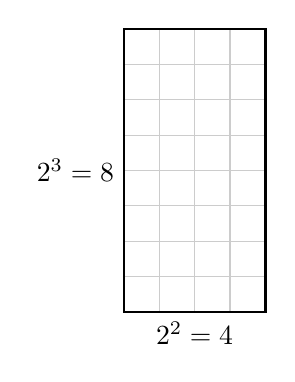
\begin{tikzpicture}[scale=0.45]
  % Grid of squares: 4 columns x 8 rows
  \draw[step=1, gray!40, thin] (0,0) grid (4,8);
  \draw[thick] (0,0) rectangle (4,8);
  \node[below] at (2,0) {$2^2 = 4$};
  \node[left] at (0,4) {$2^3 = 8$};
\end{tikzpicture}
\end{center}
\end{questionText}
\choiceA{$2^5 = 32$}
\choiceB{$2^6 = 64$}
\choiceC{$4^5 = 1{,}024$}
\choiceD{$2^{32}$}
\correctAnswer{A}
\explanation{The rectangle has $2^2$ columns and $2^3$ rows. Total squares: $2^2 \times 2^3 = 2^{2+3} = 2^5 = 32$.}
\end{practiceQuestion}

\begin{practiceQuestion}{4-7-q29}{gsa}
\begin{questionText}
A piece of paper is $0.1$ mm thick. Each time you fold it, the thickness doubles. The table shows the thickness after each fold.

\begin{center}
\begin{tabular}{|c|c|c|}
\hline
\textbf{Folds} & \textbf{Expression} & \textbf{Thickness (mm)} \\
\hline
$0$ & $0.1 \times 2^0$ & $0.1$ \\
\hline
$1$ & $0.1 \times 2^1$ & $0.2$ \\
\hline
$2$ & $0.1 \times 2^2$ & $0.4$ \\
\hline
$3$ & $0.1 \times 2^3$ & ? \\
\hline
$6$ & $0.1 \times 2^6$ & ? \\
\hline
\end{tabular}
\end{center}

Find the thickness after $3$ folds and after $6$ folds.
\end{questionText}
\correctAnswer{After $3$ folds: $0.8$ mm; after $6$ folds: $6.4$ mm}
\explanation{After $3$ folds: $0.1 \times 2^3 = 0.1 \times 8 = 0.8$ mm. After $6$ folds: $0.1 \times 2^6 = 0.1 \times 64 = 6.4$ mm.}
\end{practiceQuestion}

\begin{practiceQuestion}{4-7-q30}{gsa}
\begin{questionText}
Complete the ``exponent rule machine'' below. Write the simplified output for each input.

\begin{center}
\begin{tikzpicture}[scale=0.7]
  \node[draw, thick, rounded corners, fill=funOrange!20, minimum width=3cm, minimum height=1.2cm] at (5,0) {\textbf{Simplify}};
  % Row 1
  \node[left] at (0,2) {Input 1: $4^3 \cdot 4^5 =$};
  \node[right] at (10,2) {Output: ?};
  % Row 2
  \node[left] at (0,0.5) {Input 2: $\dfrac{7^9}{7^6} =$};
  \node[right] at (10,0.5) {Output: ?};
  % Row 3
  \node[left] at (0,-1.2) {Input 3: $(5^2)^3 =$};
  \node[right] at (10,-1.2) {Output: ?};
\end{tikzpicture}
\end{center}
\end{questionText}
\correctAnswer{$4^8$; $7^3 = 343$; $5^6 = 15{,}625$}
\explanation{Input 1: $4^{3+5} = 4^8$. Input 2: $7^{9-6} = 7^3 = 343$. Input 3: $5^{2 \times 3} = 5^6 = 15{,}625$.}
\end{practiceQuestion}
